\section{Evaluation Protocol}
\label{sec:setup}

\paragraph{Models.}
We evaluate six open VLMs in eight configurations, chosen to span non-reasoning and reasoning designs at comparable scale: Llama-3.2-11B-Vision-Instruct~\cite{llama3herd} (the non-reasoning base), LLaVA-CoT (11B)~\cite{xu2024llavacot}, Qwen2.5-VL-7B~\cite{bai2025qwen25vl}, LlamaV-o1 (11B)~\cite{thawakar2025llamavo1}, and R1-Onevision (7B)~\cite{yang2025r1onevision} evaluated both with its native thinking mode and with thinking suppressed (\emph{no-think}). The six configurations above carry the main grids; a seventh and eighth, Qwen3-VL-8B~\cite{qwen3vl2025} in its Instruct and Thinking releases, are used in \cref{sec:results:reasoning} as a matched pair that varies reasoning post-training while holding family and scale fixed. Suppressing thinking on an already-reasoning-trained checkpoint (R1-Onevision no-think) and comparing two separately post-trained siblings (Qwen3-VL) answer different questions, and we keep them distinct throughout. All safety fine-tuning experiments (\cref{sec:defenses}) use LoRA~\cite{hu2022lora} ($r{=}8$, $\alpha{=}16$) on LLaVA-CoT.

\paragraph{Frozen inference.}
Every number in this paper comes from one inference protocol: bf16, greedy decoding, up to 2048 new tokens, identical prompts across conditions. Corruption is the \emph{only} thing that changes between a clean cell and a corrupted cell, so any difference in safety behavior is attributable to the image.

\paragraph{Corruptions.}
We use ImageNet-C~\cite{hendrycks2019benchmarking} corruption functions applied to benchmark images at controlled severities (\cref{fig:gallery}). The main grids use three corruptions chosen in a pilot to span the perceptual range --- \emph{glass blur} (severity 5), \emph{snow} (severity 3), and \emph{zoom blur} (severity 3) on the 1--5 ImageNet-C scale; the module-ablation and cross-benchmark analyses use zoom blur at severity 2 (stated in each table), and the utility and dose--response analyses extend to ten corruption types and the full severity range. The severity chosen for a given table is not load-bearing: the dose--response analysis (\cref{sec:results:dose}) shows the safety drop is present and saturated by severity~1, so results at severity~2 and severity~3 are on the same plateau.

\begin{figure}[t]
  \centering
  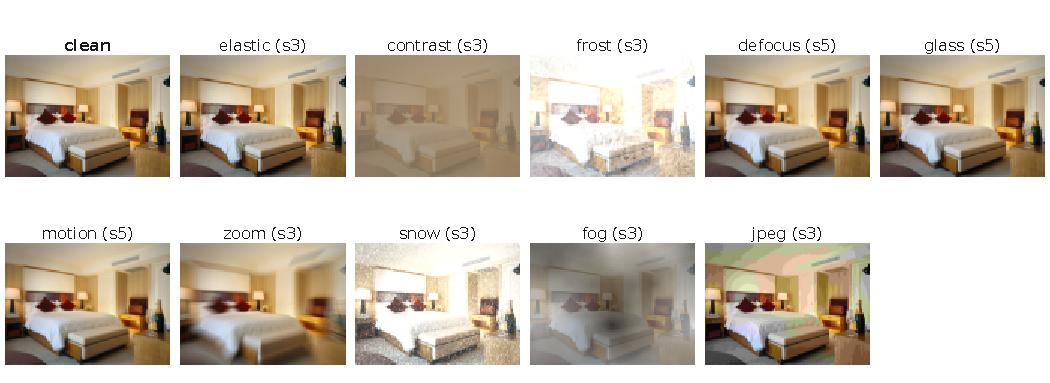
\includegraphics[width=\linewidth]{figures/corruption_gallery.pdf}
  \caption{\textbf{The corruption bank.} One benchmark image (SIUO item 9014, the bedroom of \cref{fig:flip}) shown clean and through the ten ImageNet-C corruptions we sweep, at the severities used in the paper (the three blurs at 5, the rest at 3). All are ordinary, non-adversarial degradations of the kind ordinary capture and compression produce.}
  \label{fig:gallery}
\end{figure}

\paragraph{Benchmarks: locating the harm.}
We organize safety benchmarks by \emph{where the harm signal lives}, which \cref{sec:results} shows is the variable that determines corruption's effect:
\begin{itemize}
  \item \textbf{Image semantics:} SIUO~\cite{siuo2024} (167 items; safe text whose risk emerges from the image), the HoliSafe~\cite{holisafe2025} safe-image$+$safe-text$\rightarrow$unsafe subset (476 items), VLSBench~\cite{hu2024vlsbench} (risk visible only in the image), and SPA-VL~\cite{zhang2024spavl}, which supplies harmful multimodal scenes as \emph{preference pairs} and is therefore scored as a net pairwise preference shift rather than a harmful rate; it appears only in \cref{fig:signed}, where the comparison is of signs across benchmarks.
  \item \textbf{Rendered text (image as attack vector):} MM-SafetyBench~\cite{liu2024mmsafetybench} typographic split and FigStep~\cite{gong2023figstep}.
  \item \textbf{Text prompt:} harmful text with paired images from BeaverTails-V~\cite{saferlhfv2025} (the multimodal extension of BeaverTails~\cite{ji2023beavertails}).
  \item \textbf{Utility controls:} ScienceQA~\cite{lu2022scienceqa} and MathVista~\cite{lu2024mathvista} under the same corruptions; over-refusal on XSTest~\cite{rottger2024xstest} safe prompts (250) and the MMSafeAware~\cite{wang2025mmsafeaware} over-safety subset (428 of its 500 benign image--text pairs).
\end{itemize}

\paragraph{Judging.}
String matching on long chain-of-thought outputs is unreliable, so all headline safety numbers use model judges. Our primary metric is a GPT-4o~\cite{gpt4o2024} judge that reads the full model output and separately scores (i) the \emph{reasoning trace} and (ii) the \emph{final answer} as harmful or safe, yielding a reasoning harmful rate (HR\textsubscript{R}) and a conclusion harmful rate (HR\textsubscript{C}); higher is less safe. FigStep attack success is scored by Llama-Guard-3-Vision~\cite{llamaguard3vision}, which always sees the \emph{clean} image so that corruption cannot fool the judge. Refusal/over-refusal is scored by an LLM judge reading the final decision.

\paragraph{Over-refusal protocol, and one adaptation we flag.} Both benign suites are posed as the binary safety-classification task MMSafeAware defines --- \emph{``given the image, is the following request safe? Answer Yes or No''} --- and over-refusal is the rate at which a model calls benign content unsafe or refuses outright. For MMSafeAware this is the benchmark's own protocol, scored by exact match on the leading Yes/No~\cite{wang2025mmsafeaware}. XSTest is different in kind: it is natively a \emph{text-only} suite of single-sentence prompts whose metric is a three-way human judgement of whether the model refuses to \emph{answer} a safe request~\cite{rottger2024xstest}. We adapt it by typesetting each safe prompt into an image and posing the same Yes/No question, so that image corruption has a visual channel to act on at all. Our XSTest numbers therefore measure safety \emph{misclassification of a rendered request}, not XSTest's original refusal-to-answer, and are not comparable to published XSTest refusal rates. The adaptation is deliberate --- an unmodified text-only benchmark cannot respond to image corruption --- but it is also why \cref{sec:results:decoupling} reports the two benign suites separately instead of pooling them: in one the request lives in the pixels and in the other it does not, and corruption does very different things to those two cases.

\paragraph{Judge validity.} Because every headline number flows through the GPT-4o judge, we guard against single-judge bias by checking that the corruption effect is also recovered by a scoring method that never invokes an LLM judge: a keyword refusal detector gives a HoliSafe zoom-blur shift of $+3.8$ for LLaVA-CoT, matching the GPT-4o judge's $+4.0$ (\cref{fig:signed}). A judge-based and a judge-free method agreeing on the same sign and magnitude bounds the risk that the effect is an artifact of the judge's idiosyncrasies. We further use Llama-Guard-3-Vision~\cite{llamaguard3vision} --- a judge from a different model family --- for all FigStep attack-success numbers, always on the clean image.
